\documentclass{article}
\usepackage{graphicx} % Required for inserting images

\usepackage{amsmath,amsfonts,amssymb,amsthm}
\usepackage{bm} %bold math
\usepackage{tikz}

\usepackage[margin=1.25in]{geometry}
\usepackage{parskip}

\definecolor{red}{RGB}{219,50,30}
\definecolor{pur}{RGB}{160,100,180}
\definecolor{greeo}{RGB}{91,173,69}
\definecolor{blu}{RGB}{40,120,255}

\title{Projektsammanfattning grupprojekt}
\author{
    Harry Zhang - harryz@kth.se, Mikael Häglund - mihaglu@kth.se, \\
    Carl Tang - chtan@kth.se, Anton Li - antonl8@kth.se, Aron Stålmarck - aronsta@kth.se \\
    SF 1672 - Linjär Algebra
}
\date{November 2023}

\begin{document}

\maketitle

Vi har valt ett projekt inom linjärprogrammering som handlar om att maximera avkastningen från ett jordbruk. Problemet är även känt som “Farmer’s problem”.

Mer specifikt:

Exempel på givna parametrar:
\begin{itemize}
    \item Total brukbar landyta
    \item Total budget
    \item Olika antal grödor, som i sin tur har parametrar som:
    \begin{itemize}
        \item Avkastning per landyta
        \item Försäljningspris
        \item Pris för att plantera
        \item Minimal och maximal mängd som får plantera
    \end{itemize}
\end{itemize}

Den bakomliggande teorin för problemet är att alla begränsningar på parametrarna (olikheter) är linjära, vilket gör problemet till ett som kan lösas med linjärprogrammering. Lösningsmängden för alla parametrar kommer att bilda en polytop i $\mathbb{R}^n$ (om $n$ är antalet parametrar) och en optimal lösning för avkastningen kommer att ligga i ett hörn av polytopen. En algoritm för att hitta denna optimala lösning kallas simplexmetoden.

\begin{figure}[h]
\centering
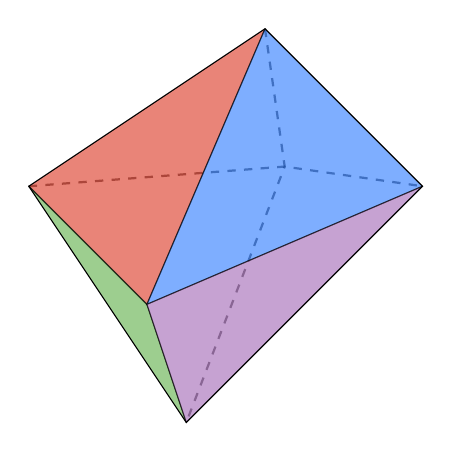
\begin{tikzpicture}[scale=5]
\coordinate (A1) at (0.1,0.1);
\coordinate (A2) at (0.75,0.15);
\coordinate (A3) at (1.1,0.1);
\coordinate (A4) at (0.4,-0.2);
\coordinate (B1) at (0.7,0.5);
\coordinate (B2) at (0.5,-0.5);

\begin{scope}[thick,dashed,,opacity=0.6]
\draw (A1) -- (A2) -- (A3);
\draw (B1) -- (A2) -- (B2);
\end{scope}
\draw[fill=red,opacity=0.6] (A1) -- (A4) -- (B1);
\draw[fill=greeo,opacity=0.6] (A1) -- (A4) -- (B2);
\draw[fill=blu,opacity=0.6] (A3) -- (A4) -- (B1);
\draw[fill=pur,opacity=0.6] (A3) -- (A4) -- (B2);
\draw (B1) -- (A1) -- (B2) -- (A3) --cycle;
\end{tikzpicture}
\caption{En polytop motsvarar lösningsmängden - en optimal lösning kommer alltid finnas i ett hörn.}
\end{figure}

\begin{tikzpicture}[scale=2]
\coordinate (O) at (0,0);
\coordinate (A1) at (0,3);
\coordinate (A2) at (0.6,3.5);
\coordinate (A3) at (1.6,3.3);
\coordinate (A4) at (3.4,2.3);
\coordinate (A5) at (4.3,0);

\coordinate (L1) at (-0.15,5.85);
\coordinate (L2) at (5.85,-0.15); % slope is -1

\coordinate (P) at (2.85,2.85);
\coordinate (Q) at (3.65,3.65);

\draw[blue] (O) -- (A1) -- (A2) -- (A3) -- (A4) -- (A5) -- (O);
\draw[red] (L1) node[above]{$Z(x)=c$} -- (L2);
\draw[->] (P) -- (Q);
\end{tikzpicture}

\begin{align*}
&\text{Maximera} \ Z(\bm{x}) := \bm{c}^T\bm{x} \\
&\text{under begränsningarna} \ A\bm{x} \le \bm{b} \ \text{och} \ \bm{x} \ge 0.
\end{align*}



\section*{Stegen i Simplexmetoden}
\begin{enumerate}
    \item \textbf{Formulera Problem:} Omvandla optimeringsproblemet till standardform, där alla begränsningar är likheter och målfunktionen är en maximeringsfunktion. Alla variabler måste vara större eller lika med noll.
    
    \item \textbf{Konstruera Simplex-tabell:} Skapa en initial simplex-tabell (matris) som representerar alla ekvationer och målfunktionen. Lägg till en slackvariabel för varje olikhet för att göra det till en likhet.
    
    \item \textbf{Identifiera Pivotkolonn:} Välj en icke-basvariabel (oftast den med det största negativa koefficienten i målfunktionsraden) för att introducera i lösningens bas.
    
    \item \textbf{Identifiera Pivotelement:} Använd pivoteringsregler för att bestämma vilken basvariabel som ska tas bort (raden med minst kvot när man dividerar sista elementet med elementet i pivotkolonnen är pivotraden, och elementet blir pivotelementet).
    
    \item \textbf{Pivotera:} Utför räkneoperationer för att uppdatera tabellen med den nya basvariabeln (Gauss-Jordan elimination).
    
    \item \textbf{Kontrollera Optimalitet:} Kontrollera om den nuvarande lösningen är optimal.
    \[
    \text{Om alla } x_j \geq 0, \text{ är lösningen optimal.}
    \]
    
    \item \textbf{Upprepa Vid Behov:} Om lösningen inte är optimal, börja om från steg 3 och upprepa processen.
\end{enumerate}

Vi kommer använda oss av ett specifikt fall av Farmer’s problem, men kan även generera egen testdata av olika storlekar som vi kan testa vår algoritm på. 

Frågeställningen är därmed: Hur mycket av varje gröda ska vi köpa/plantera för att maximera avkastningen givet de olika kraven?

Möjliga tillämpningar av detta finns även i verkligheten, (då den heter bondens problem bokstavligt talat) då den återfinns på i princip alla bondgårdar/jordbruk när det kommer till att maximera avkastningen och effektiviteten givet vissa krav på produktionen. Med vårt program kommer vi ha med ett par av de vanligare kraven som man behöver ta hänsyn till men det finns givetvis flera variabler och begränsningar man skulle kunna lägga till.

\end{document}


